\section{Retransmission Response Packet Processing Module}

The Retransmission Request Packet Processing module takes an input
retransmit request and attempts to acquire the requested packet from the RETX interface. It then sends
that packet out to the interface. Note that the packet retrieved from
the FIFO may not be the packet requested, if the FIFO has since
wrapped around.

\subsection{Implementation}

A successful packet lookup is detected by correctly acquiring the
sequence number and storing it in \signal{LOOKUPSEQ[31:0]}. A success
results in the assertion of \signal{RETXSUCCESS}. A failed look-up (in
which we do not find a packet with a completely-matching sequence ID)
causes the assertion of a \signal{PKTNOTINBUF}. These signals are used
by external counters to measure retx success.


\begin{figure}
\begin{centering}
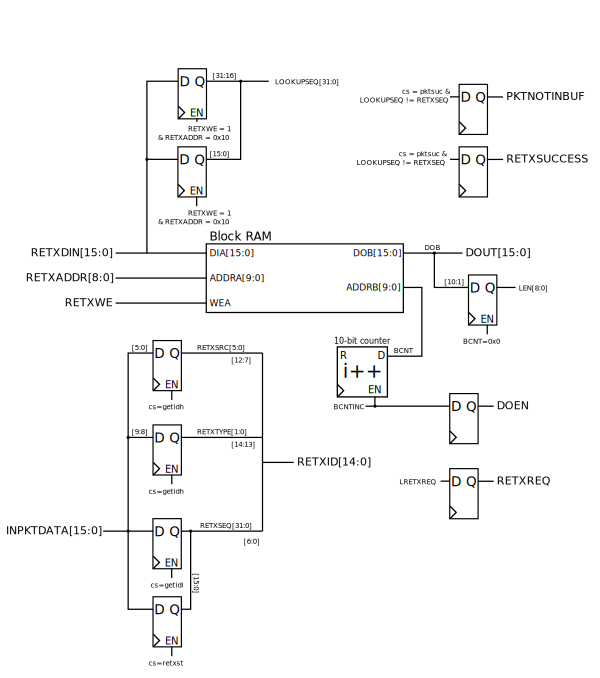
\includegraphics[scale=0.8]{dataretxresponse.svg}
\end{centering}
\caption{Data Retransmission Request module.}
\label{dataretxresponse}
\end{figure}

\begin{figure}
\begin{centering}
\includegraphics[scale=0.8]{dataretxresponse.fsm.svg}
\end{centering}
\caption{Data Retransmission Request module FSM.}
\label{dataretxresponse.fsm}
\end{figure}
